\documentclass[tikz]{standalone}%

\usepackage[utf8]{inputenx}%  http://ctan.org/pkg/inputenx
% Euler for math | Palatino for rm | Helvetica for ss | Courier for tt
\renewcommand{\rmdefault}{ppl}% rm
\linespread{1.05}% Palatino needs more leading
\usepackage[scaled]{helvet}% ss //  http://ctan.org/pkg/helvet
\usepackage{courier}% tt // http://ctan.org/pkg/courier
\usepackage{eulervm}  %  http://ctan.org/pkg/eulervm
% a better implementation of the euler package (not in gwTeX)
\normalfont%
\usepackage[T1]{fontenc}%  http://ctan.org/pkg/fontenc
\usepackage{textcomp}%  http://ctan.org/pkg/textcomp

\usetikzlibrary{angles}
\usetikzlibrary{quotes}
\usetikzlibrary{calc}
\usetikzlibrary{intersections}

\begin{document}
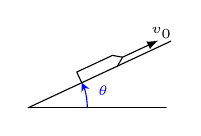
\begin{tikzpicture}[line cap = round, line join = round]
  \draw (0, 0) coordinate (O) -- (25:2cm) coordinate (A);
  \draw (O) -- (1.75cm, 0) coordinate (B);

  \path (B) -- (O) -- (A) pic["$\theta$", angle radius = 0.75cm,
  angle eccentricity = 1.3, blue, draw, -stealth, font = \tiny]
  {angle = B--O--A};
  
  \draw (25:0.75cm) coordinate (P1) -- ($(P1)!0.15cm!-90:(O)$) coordinate
  (P2) -- ++(25:0.5cm) coordinate (P3);

  \path[name path = line] ($(P1)!.50!(P2)$) -- ++(25:0.7cm);
  \path[name path = aline] (P3) -- ++(-10:0.2cm);
  \path[name intersections = {of = line and aline, by = P4}];

  \draw (P3) -- (P4);
  \draw (P4) -- (25:1.25cm);
  \draw[-latex] (P4) -- ++(25:0.5cm) node[font = \tiny, pos = 1.1, above,
  inner sep = 0.1] {$v_0$};
\end{tikzpicture}
\end{document}
%%% Local Variables:
%%% mode: latex
%%% TeX-master: t
%%% End:
